\documentclass [11 pt, oneside] {article}


\def \jtitle {Lie groups}
\def \jlecturer {Richard Borcherds}
\def \jterm {}
\def \jauthor {Jack DeSerrano}


\usepackage [course] {jack}

\title {Lie groups}
\author {Jack DeSerrano}

\begin {document}

\maketitle

These notes are based on Richard Borcherds's YouTube series on Lie groups.\footnote{See \url{https://www.youtube.com/playlist?list=PL8yHsr3EFj53RWBkiHKoOsTw-dGHAoJ-h}.}

\begin {figure}
	\begin {center}
		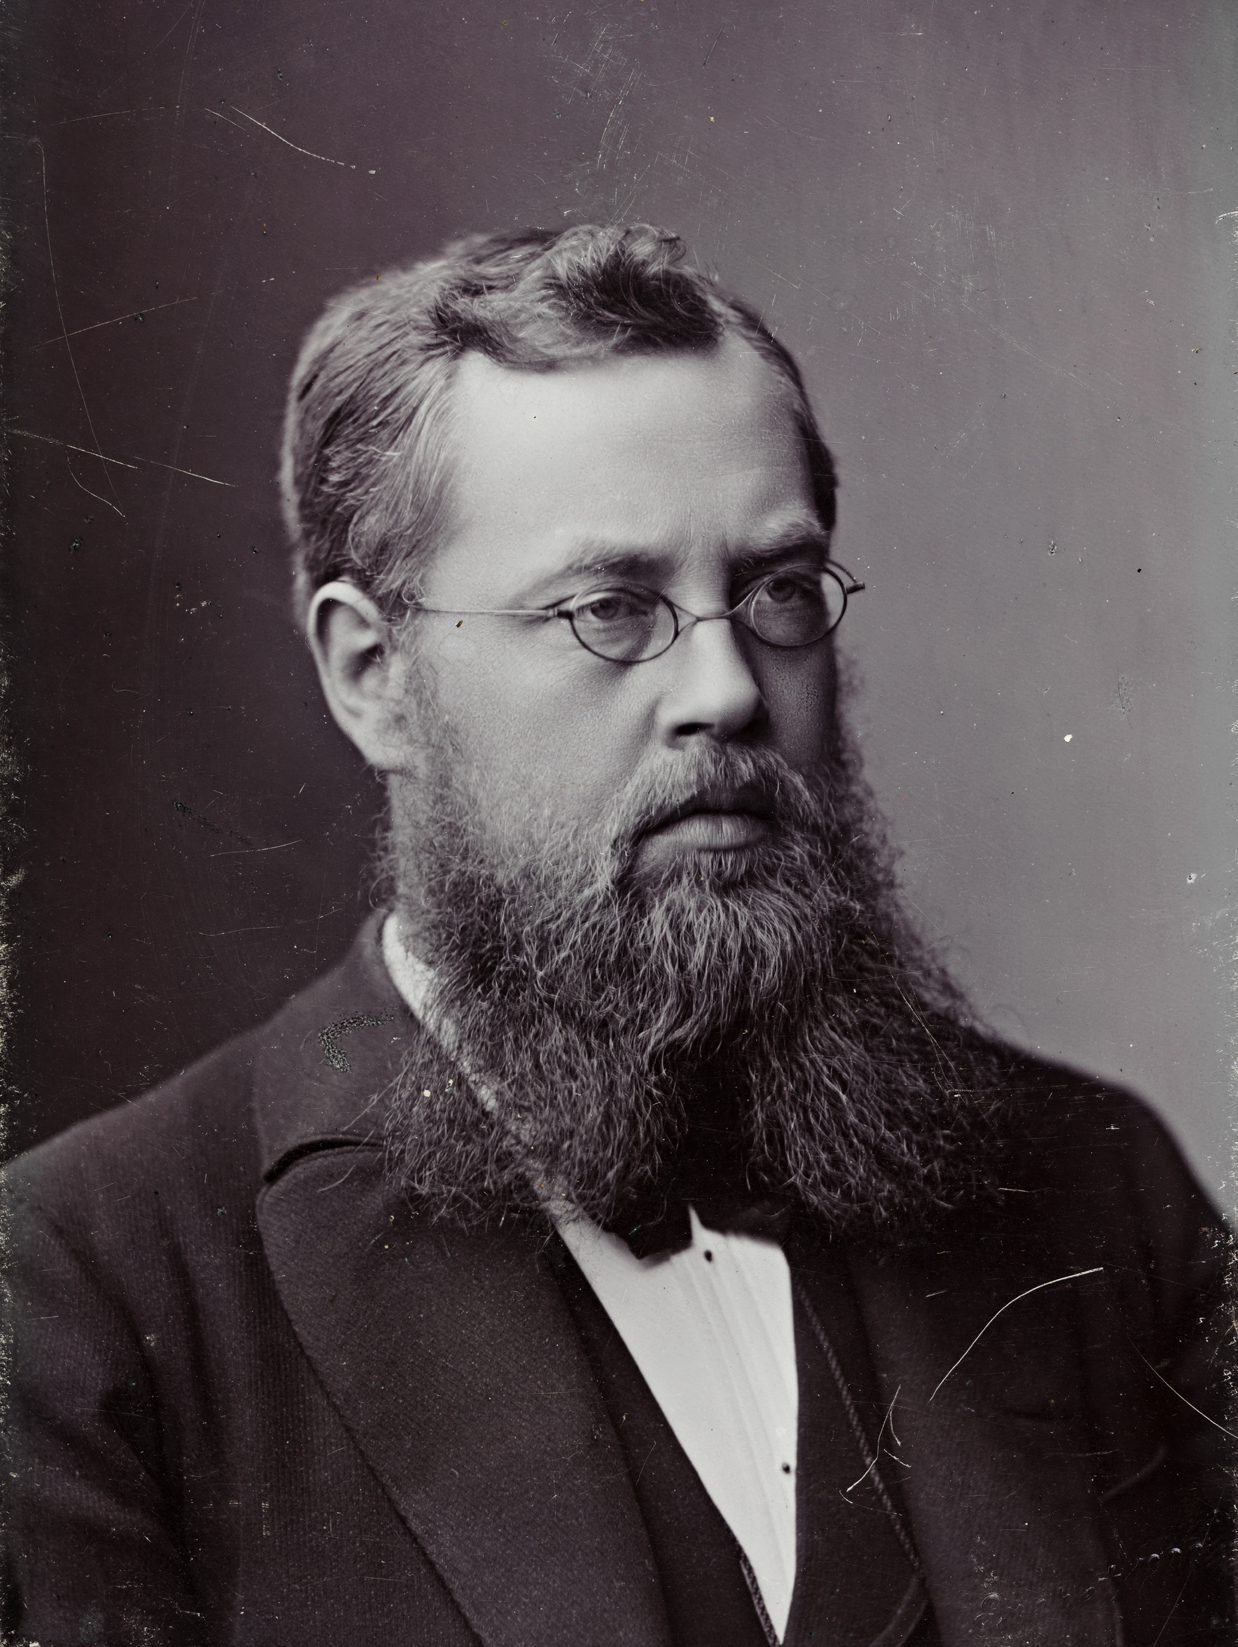
\includegraphics [scale = 0.33] {images/lie}
		\caption {Sophus Lie.}
	\end {center}
\end {figure}
% https://upload.wikimedia.org/wikipedia/commons/a/a3/Portrett_av_Sophus_Lie.jpg
% https://www.flickr.com/photos/48220291@N04/8447487830

\newpage

\iffalse
	\hypersetup {linkcolor = black}
	\tableofcontents
	\hypersetup {linkcolor = Red}
\fi

\section {Introduction}
First thing's first:
\begin{align*}
	\textrm{Lie} = \textrm{li\textlengthmark}
\end{align*}

A \defn{Lie group}\index{Lie group} is a group and a manifold, so, locally, it looks like $\mathbf{R}^{n}$. The number $n$ is the \defn{dimension}\index{dimension of a Lie group} of the Lie group.

The group $\GL_{n}(\mathbf{R})$ is a Lie group of dimension $n^{2}$: It is an open subset of the space of $n\times n$ matrices. 

Lie groups of dimension $0$ are, essentially, the same as discrete groups.
The classification of discrete groups is completely hopeless.
However, any Lie group $G$ has a connected component $G\sub{con}$ that is a normal subgroup of $G$.\footnote{This group is also a Lie group.}
The quotient $G\sub{disc} = G/G\sub{con}$ is $0$-dimensional.
Thus, one can split a Lie group into a discrete part and a connected part. One can, more or less, classify the connected Lie groups.

\begin{example}[ ]\label{}\text{}
Take $G:= \mathbf{R}^{*}$. 
Then, $G\sub{con} = \mathbf{R}_{>0}$ is the connected part and $G\sub{disc} = \{+,-\}$ is the discrete part.
\end{example}

The groups $\mathbf{R}$ under addition, $\mathbf{R}^{*}$ under multiplication, and $S^{1}\subset \mathbf{C}^{*}$ are $1$-dimensional Lie groups.
There are group homomorphisms
\[
\begin{tikzcd}
	\exp:\mathbf{R}\ar[r] & \mathbf{R}^{*}
\end{tikzcd}
\]
and
\[
\begin{tikzcd}
	\mathbf{R}^{*}\ar[r] & S^{1} : z\ar[r,mapsto] & e^{2\pi i z}.
\end{tikzcd}
\]
The second homomorphism is a \defn{local isomorphism}\index{local isomorphism}.
Any connected $1$-dimensional Lie group is isomorphic to $\mathbf{R}$ under addition or $S^{1}$ under multiplication.

Clearly, $\mathbf{R}^{1}\times \mathbf{R}^{1} = \mathbf{R}^{2}$, $\mathbf{R}^{1}\times S^{1}$, and $S^{1}\times S^{1}$ are $2$-dimensional Lie groups. 
Each of these Lie groups is of the form $\mathbf{R}^{2}/G\sub{disc}$ where $G\sub{disc}$ is a discrete group.\footnote{This group is $0$, $\mathbf{Z}$, or $\mathbf{Z}^{2}$.}
Any abelian connected Lie group is isomorphic to
\begin{align*}
	\mathbf{R}^{m} \times (S^{1}) ^{n} \isomto \mathbf{R}^{m+n}/G\sub{disc}
\end{align*}
where $G\sub{disc}$ is a discrete group.

There are no nonabelian connected Lie groups of dimension $1$. 
However, the $az+b$ group is a connected Lie group of dimension $2$, and one can see that it is nonabelian. Nevertheless, it is a \defn{solvable Lie group}\index{solvable Lie group}: That is, there is a chain of Lie groups
\begin{align*}
	1 = G_0 \subset \cdots \subset G_{n} = G
\end{align*}
where $G_{i}/G_{i-1}$ is abelian.

The group $\SL_{2}(\mathbf{R})$ is a dimension-$3$ Lie group. From this, one gets the $3$-dimensional Lie group
\begin{align*}
	\PSL_{2}(\mathbf{R}) = \SL_{2}(\mathbf{R}) / \left\{ \pm 1 \right\}.
\end{align*}
This is the group $\Aut(\mathfrak{H})$ via the action
\begin{align*}
	\mat{a&b\\c&d}(\tau) =  \frac{a\tau+b}{c\tau+d}.
\end{align*}
The group $S^{3}$, which one can think of as the unit quaternions, is a $3$-dimensional Lie group.\footnote{The sphere $S^{n}$ is a Lie group for $n=0,1,3$.}

The \defn{Heisenberg group}\index{Heisenberg group} 
\begin{align*}
	\underbrace{\mat{1&a&b\\&1&c\\&&1} }_{\mathbf{R}^{3}} / \underbrace{\mat{1&0&n\\&1&0\\&&1}}_{\mathbf{Z}} 
\end{align*}
is a Lie group of dimension $3$.\footnote{This is an example of taking a Lie group and modding out by a discrete subgroup of its centre.}
One can transform a function via
\[
\begin{tikzcd}[row sep = 0 em]
	f(z) \ar[r,mapsto] & f(z+a);\\
	f (z) \ar[r,mapsto] & e ^{icz}f(z);\\
	f (z)\ar[r,mapsto] & \alpha f (z);
\end{tikzcd}
\]
where $\left\lvert \alpha \right\rvert =1$.
These transformations correspond to elements of the Heisenberg group.
While $\mathbf{R}^{3}$ is simply connected, the Heisenberg group isn't. Nevertheless, its fundamental group is $\mathbf{Z}$.

One can reduce the classification of Lie groups to the classification of simply connected Lie groups: Any Lie group is a simply connected Lie group modulo a discrete subgroup of its centre. 

The Heisenberg group is \defn{nilpotent}\index{nilpotent group}. More generally, any group
\begin{align*} % https://tex.stackexchange.com/questions/17416/create-a-new-integral-symbol/17419#17419
	\mat{1&*&&*&*\\
		      &1&*& \hbox to .2em{\hss\scalebox{1}[1] {\rotatebox[origin=c]{90}{$\ddots$}}\hss} &*\\
		      &&\ddots&\ddots\\
		      &&&1&*\\
		      &&&&1} 
\end{align*}
is nilpotent.

The \defn{Lorentz group}\index{Lorentz group} $\O_{1,3}(\mathbf{R})$ is the group of rotations of spacetime: The group of linear operators on $\mathbf{R}^{4}$ that preserve the quadratic form
\[
\begin{tikzcd}
	(z_1,z_2,z_3,z_4)\ar[r,mapsto]& z_1^{2} - z_2^{2}-z_3^{2}-z_4^{2}.
\end{tikzcd}
\]
The Lorentz group is a $6$-dimensional Lie group that has a nontrivial fundamental group.
It has $4$ components: One can reverse time and reverse space.
Physicists believed that all physical theories were invariant under time reversal and space reversal. However, the weak interaction is not invariant under space inversion. Things do not need to be invariant under time inversion, either. 

The connected component of $\O_{1,3}(\mathbf{R})$ has a double cover $\Sp_{1,3}(\mathbf{R})$ called a \defn{spin group}\index{spin group}.
The group $\Sp_{1,3}(\mathbf{R})$ is locally isomorphic to $\SL_{2}(\mathbf{C})$, which has $2$-dimensional representations that $\O_{1,3}(\mathbf{R})$ does not have. This causes the existence of fermions and electrons.
This local isomorphism is an example of an ``accidental isomorphism.'' There are many ``accidental isomorphisms'' between Lie groups of small dimensions.

The group $\SU_3$ is an $8$-dimensional Lie group. This group is the gauge group of quantum chromodynamics and is involved in the flavour symmetries of old theories of the strong interaction.\footnote{Murray Gell-Mann called it the ``eightfold way.''}
This is a \defn{simple Lie group}\index{simple Lie group}: That is, it has no nontrivial connected normal subgroups.

The \defn{Poincar\'e group}\index{Poincar\'e group} $\mathbf{R}^{1,3} \rtimes \O_{1,3}(\mathbf{R})$ is a $10$-dimensional Lie group.
The Lie group $\mathbf{R}^{1,3}$ is solvable and the Lie group $\O_{1,3}(\mathbf{R})$ is a product of simple Lie groups.

Complex simple Lie groups are complex manifolds, not real manifolds. Examples of these include $\SL_{n}(\mathbf{C})$ for $n\ge 1$, $\O_{n}(\mathbf{C})$ for $n\ge 3$, and $\Sp_{2n}(\mathbf{C})$ for $n\ge 1$. These are the \defn{classical groups}\index{classical group} over $\mathbf{C}$.
Wilhelm Killing added $5$ more to this list:
\begin{center}
\begin{tabular}{ll}
    Group & Dimension\\
    \midrule
    G_2 & 14\\
    F_4 & 52\\
    E_6 & 78\\
    E_7 & 133\\
    E_8 & 248
\end{tabular}
\end{center}
Dr. Borcherds remarks:
\begin{quote}
	\small Killing really ought to be a lot better known. He was a kind of really modest, shy guy and invented a lot of things that were later named after other people. Later on in this course, we will be talking about the Weyl group, the Coxeter number, the Cartan form, and things like that, and these were all actually first invented by Killing and people kind of forgot he invented them.
\end{quote}

\iffalse
\section {Lie algebras}

\section {Lie groups and Lie algebras}

\section {The exponential map}

\section {The Poincar\'e--Birkhoff--Witt theorem}

\section {The Baker--Campbell--Hausdorff formula}

\section {Positive characteristic is weird}

\section {Bianchi classification}

\section {Engel's theorem}

\section {Lie's theorem}

\section {The Haar measure}
\fi

\printindex

\end {document}
